\chapter{Commande d'un drone à aile libre rotation libre}
\minitoc

\section{Inversion non linéaire incrémentale de la dynamique du drone}
The theory of Incremental Nonlinear Dynamic Inversion (INDI) used in the context of micro-UAVs is presented in \cite{smeurINDI}. We use the notation proposed in \cite{smeurINDITail}, without providing extra details, due to length constraints. The central underlying assumption is that the so-called timescale separation principle holds w.r.t. the actuator dynamics and the dynamics of aerodynamic forces and moments. The control signal can then be computed incrementally using the actuator effectiveness matrix $G$.
\begin{align}
    u_{\text{W}} = u_{\text{W}} + G^{\dag} (\nu - \begin{bmatrix}
    \dot{\omega}_{\text{W}} \\
    T_{\text{W}}
    \end{bmatrix})
\end{align}
where $ \dot{\omega}_{\text{W}} \in \real^{3}$ is the measured angular acceleration obtain by finite difference from equation (\ref{eq:gyro_deplacement}), $T_{\text{W}} \in \real$ is the current thrust, $\nu$ is define in \cite[equation (4)]{smeurINDITail} and $G$ is the control effectiveness matrix, determined as follows :
\begin{align*}
    \begin{bmatrix}
    \partial \phi \\
    \partial \theta \\
    \partial \psi \\
    \partial T
    \end{bmatrix}\! =\! G u_{f} \!=\!
    \begin{bmatrix}
    -7.5 & -15 & 7.5 & 15 & 0 & 0\\
    0 & 0 & 0 & 0 & 15 & 15 \\
    0 & 0 & 0 & 0 & 4 & -4 \\
    -0.6 & -0.6 & -0.6 & -0.6 & 0 & 0\\
    \end{bmatrix}
    u_{f}
\end{align*}
This selection of efficiency matrix has been determined for the hovering flights, but it is necessary to carry out a different study for the forward flight.


To stabilise the fuselage, we use a PD feedback from the angle $\theta_{\text{F}}$ formed between the fuselage and the horizontal, which we want to keep at zero. This is obtained by converting the quaternion $q_{\text{F}}$ of equation (\ref{eq:quat_fuselage}) into an Euler angle by following the 'ZYX' Euler convention. The PD feedback provides the reference $u_{\text{tail}}$ for the angular speed of the motor generating the force $F_{m}$ (see Figure  \ref{fig:colibri_frame_side}), as follows
\begin{align*}
    u_{\text{tail}} = u_{eq} + k_{p} \theta_{\text{F}} + k_{d} \dot{\theta_{\text{F}}},
\end{align*}
where $u_{eq}$ is the equilibrium motor command to keep the fuselage horizontal in the absence of disturbance and $k_{p}$, $k_{d}$ are tunable scalar gains. The value $u_{eq}$ was obtained by applying a moment theorem to the fuselage at the point $O_{\text{W}}$. In fact, the two moments that come into effect on the fuselage are the torque due to the thrust force of the tail motor and the torque due to the position of the fuselage's centre of gravity.
The gains $k_{p}$ et $k_{d}$ were adjusted in flight to ensure satisfactory flight behaviour. We obtain $\dot{\theta_{\text{F}}}$ from $\omega_{gyro}^{F} = [\dot{\phi_{\text{F}}}~\dot{\theta_{\text{F}}}~\dot{\psi_{\text{F}}}]^\top$.
\section{Experimentation}
\label{sec:exp}
% \todo{Photo de la volière: It is difficult to understand the experimental results
% due to the absence of snapshots, detailed explanations, or
% pictures of the experimental environment. Illustrations and
% explanations of the experimental structure, actual flight
% photos, and the design structure of the entire flight
% system must be added.}
An experimental prototype was developed, as shown in Figure~\ref{fig:colibri_real}. A selection of the experimental results in controlled flight is shown in Figure \ref{fig:colibri_flight}.\\
\begin{figure}[!h]
    \centering
    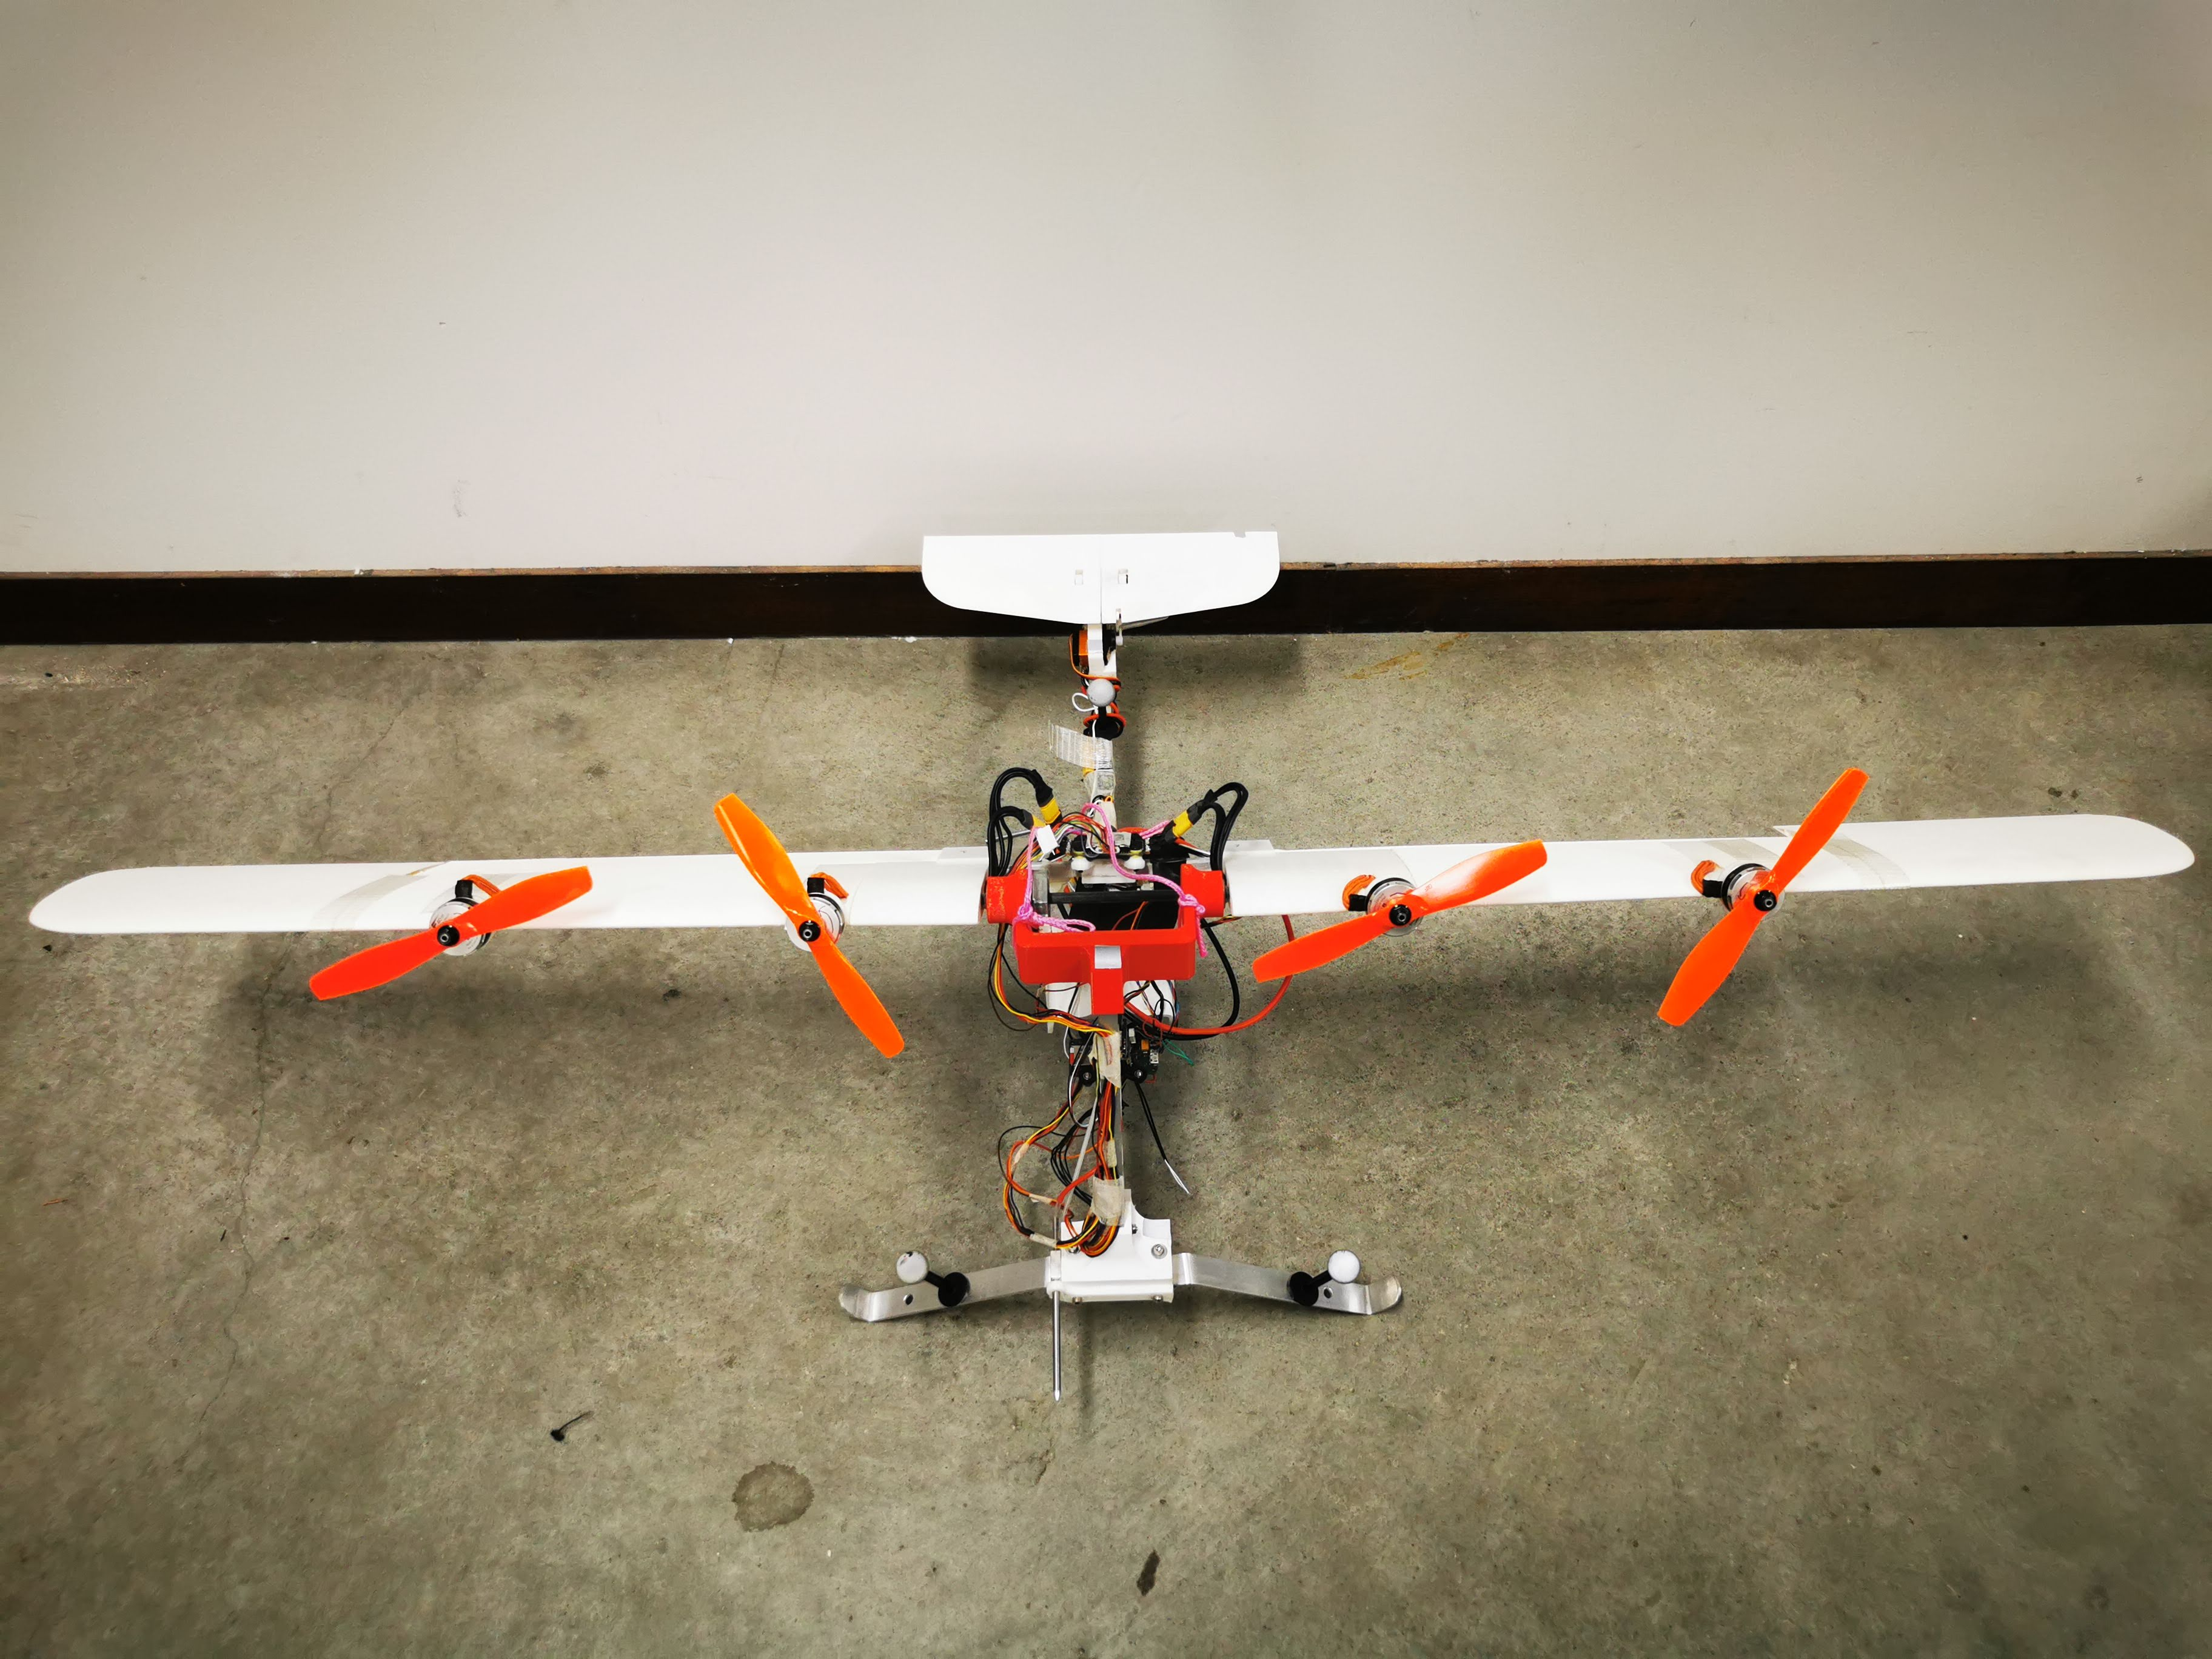
\includegraphics[trim={0 15cm 0 25cm},clip, width=\columnwidth]{figures/colibri_real.jpg}
    \caption{Colibri experimental prototype.}
    \label{fig:colibri_real}
\end{figure}
About Figure \ref{fig:colibri_flight}, from \SI{0}{\second} to \SI{8}{\second}, the drone is on the ground. From \SI{8}{\second} to \SI{16}{\second}, the drone takes off to reach a height of 2 metres visible from the third plot. This height is reached after a 10 \% overshoot. The drone is held in this position for \SI{54}{\second}. Incidence oscillations are observed in the fifth and last plot, generating oscillations in the drone's horizontal position. This is due to the coupling between the two bodies, which is not properly stabilized. From \SI{70}{\second}, the UAV starts heading towards the point $p_{c} = \begin{bmatrix} 3 & 0.9 & -1.5 \end{bmatrix}^\top$ and $\psi_{c}=\SI{90}{\degree}$.
%This brings the drone in front of the WindShape open wind tunnel. The wind generator is switched on at \SI{95}{\second} at a speed of \SI{1}{\per\second}. This disturbance destabilises the drone, which is not shown here. \todo{GH: ça fait beaucoup d'info qui ne seront pas détaillés, est-ce qu'il faut tout garder ?}
\begin{figure}[h]
\centering
    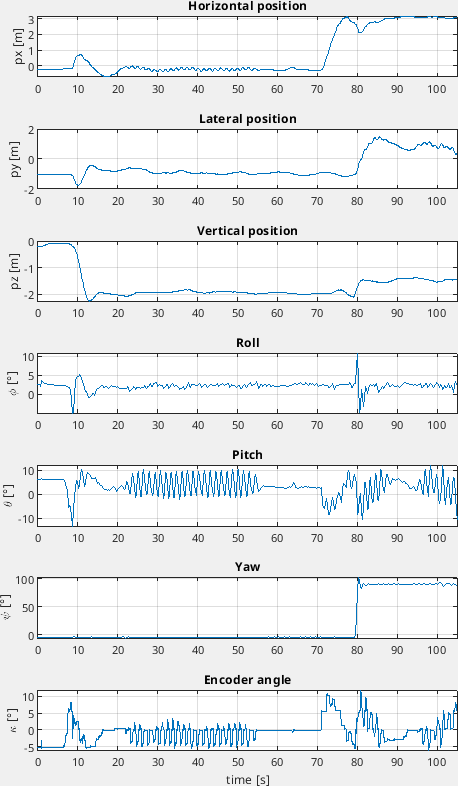
\includegraphics[width=1\columnwidth,angle=0]{figures/colibri_flight.png}
    \caption{Position and orientation of the reference frame wing in the first six graphs and pivot angle measurement on the last graph below during real flight. }
    \label{fig:colibri_flight}
\end{figure}

\section{Commande Udwadia-Kalaba}

\section{Vols expérimentaux}







